% Imporditud: tools/import_eksperimendid.py
% Allikas: Eesti füüsikaolümpiaadi eksperimendi ülesannete
%   kogu (Rael Kalda, 2023), ülesanne Ü107, lahendus L107.
\setAuthor{EFO žürii}
\setRound{lõppvoor}
\setYear{2013}
\setNumber{G E1}
\setDifficulty{3}
\setTopic{elektriahelad}
\setVahendid{takistitest tähtühendus, patarei, voltmeeter. Mõõtemääramatusi hinnata pole vaja}
\setPunktid{12}
\setAllikas{Eksperimendi kogu Ü107, lahendus lk 81}
\setLahendusseis{toores}

\prob{Täht}
Kolmest takistist on joonisel kujutatud viisil moodustatud tähtühendus. Tähe
harudest väljuvad skeemil kujutatud värvi juhtmed ning tähe keskpunkt on
isolatsiooniga kaetud.

\osa Mõõtke takistite $R_{\mathrm{K}}$, $R_{\mathrm{R}}$ ja $R_{\mathrm{P}}$
takistuste suhted neist vähimasse eeldades, et voltmeeter on ideaalne.

\osa Hinnake takistite takistusi, kui on teada, et voltmeetri takistus on
$\SI{4500}{\ohm}$.

\begin{center}
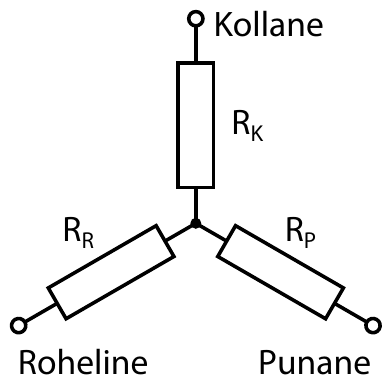
\includegraphics[width=0.30\linewidth]{2013-v3g-ge1-yl.png}
\end{center}

\hint

\solu
a) (8 p) Ühendame patarei tähe kahest tipust tulevate juhtmetega (olgu need näiteks roheline ja kollane). Sel juhul on takistid RR ja RK patareiga jadamisi ühendatud ning mõlemat takistit läbib võrdse tugevusega vool. Mõõdame nendele takistitele langevad pinged UR ja UK , ühendades voltmeetri esmalt kollase ning punase ning seejärel rohelise ning punase juhtmega. Kuna siin eeldame, et voltmeeter on ideaalne, siis punase juhtmega takistit vool ei läbi ning temale pinget ei lange. Seetõttu saame mõõtmistest otse teada pinge kollase ning rohelise juhtmega takistitel. Ohmi seaduse järgi kehtib võrdsete voolutugevuste korral seos

RR = UR . RK UK

Seega annab mõõdetud pingete jagatis takistuste RR ja RK suhte. Kui kordame samu mõõtmisi veel kaks korda, siis saame takistuste suheteks

RR $\approx$ 2, RP $\approx$ 2, RP $\approx$ 4. RK RR RK

Nagu näha, siis on väikseima väärtusega takisti RK ja vastuseks anname kõigi takistite väärtused just tema takistuse suhtes: RKs = 1, RRs = 2 ja RP s = 4.

b) (4 p) Takistuste absoluutväärtuste määramiseks leiame nende seose voltmeetri takistusega. Esmalt mõõdame patarei klemmipinge U koormamata olukorras. Järgmisena koormame patarei tähe kahe haruga ja mõõdame uuesti klemmipinge. Nagu näeme, siis voltmeetri näit võrreldes koormamata juhuga praktiliselt ei lange, mis tähendab, et pingeallika sisetakistusega pole vaja arvestada. Teatavasti saab reaalset voltmeetrit kujutada kui lõpmatu takistusega ideaalset voltmeetrit,

millega on rööbiti ühendatud reaalse voltmeetri takistusega võrdse väärtusega takisti. Ühendame nüüd jadamisi patarei, voltmeetri ja tähe kaks haru. Voltmeeter mõõdab nüüd pinget UV omaenda takistil. Jadaühenduses jaotub patarei pinge

U = UR1 + UR2 + UV ,

kus UR1 ja UR2 on patareiga ühendatud tähe harudele langevad pinged. Seega UR1 + UR2 = U $-$ UV ja jällegi Ohmi seadus rakendades saame

$R_1$ + $R_2$ = U $-$ UV , RV UV

kus RV on voltmeetri takistus. Nagu näha on mõõdetavate suuruste U ja UV vahe suurim ja tulemus täpseim, kui kasutada kahte suurema väärtusega takistit. Ülesande a-osast teame, et RR = 2RK ja RP = 4RK , millest saame arvutada

RK = RV (U $-$ UV ) 6UV .

Kuna RV = 4500 $\Omega$ ja tüüpiliselt U $\approx$ 5,8 V ning UV $\approx$ 5,3 V, siis saame takistite väärtusteks RK $\approx$ 70 $\Omega$, RR $\approx$ 140 $\Omega$ ja RP $\approx$ 280 $\Omega$.
\probend
